\RequirePackage{shellesc}
\immediate\write18{tex braids_code.dtx}
\documentclass{article}

\usepackage{tikz}
\usetikzlibrary{
  braids,
  arrows.meta
}

\begin{document}
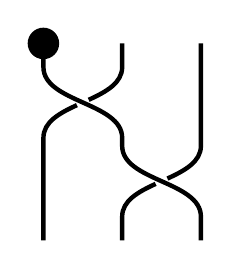
\begin{tikzpicture}[ultra thick]
\pic[name prefix=braid] {braid={s_1 s_2}};
\fill (braid-1-s) circle[radius=2mm];
\end{tikzpicture}
\end{document}

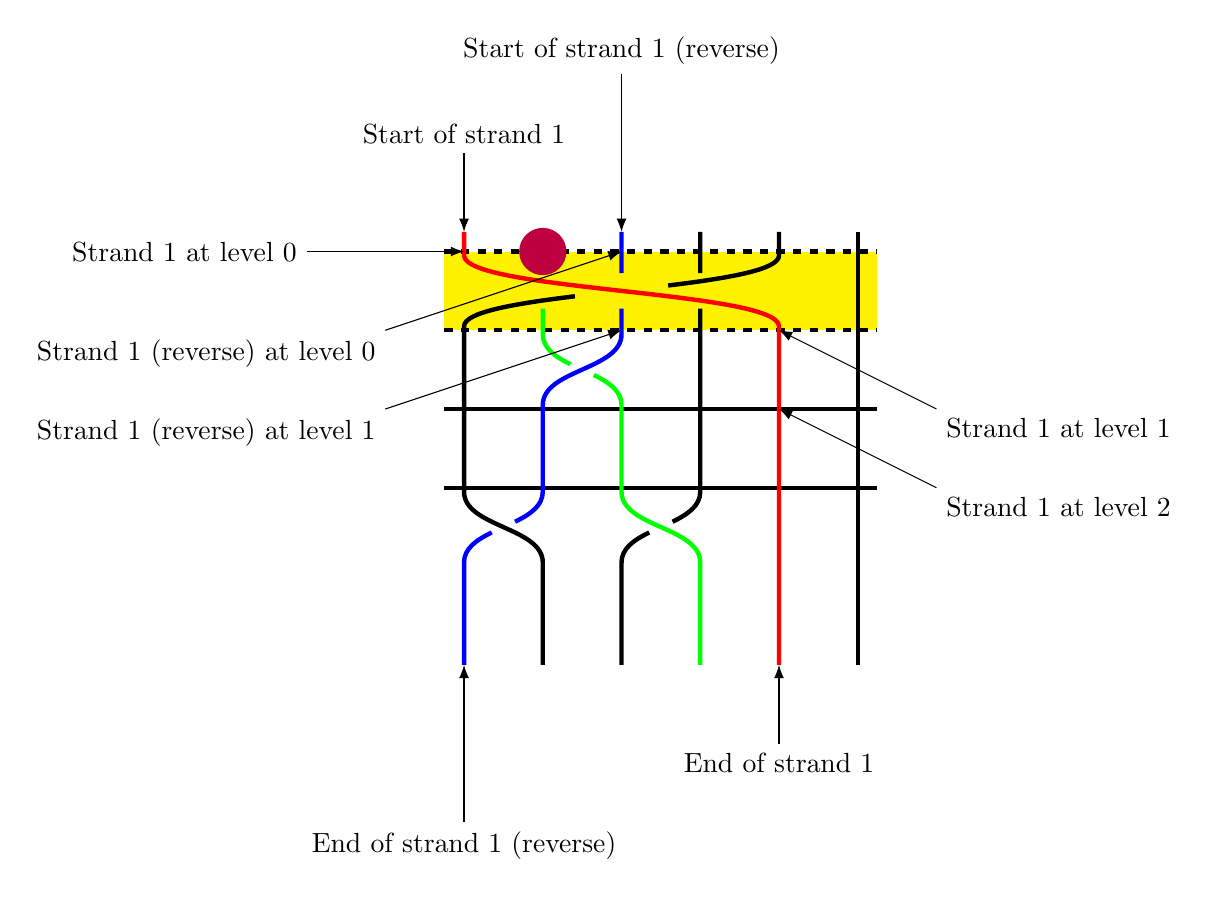
\begin{tikzpicture}[>=Latex]
\pic[
  ultra thick,
  braid/strand 1/.style={red},
  braid/strand 2/.style={green},
  braid/strand 3/.style={blue},
  braid/every floor/.style={draw=black},
  braid/floor 1/.style={fill=yellow,dashed},
  braid/number of strands=6,
  braid/width=1cm,
  braid/gap=.1,
  braid/anchor=2-0,
  name prefix=braid,
] {braid={|s_{1,5} s_2^{-1} | 1 s_3-s_1 1}};% s_2 | s_1^{-1}-s_3 | 1 s_1}};
\draw[<-] (braid-1-e) -- +(0,-1) node[below] {End of strand 1};
\draw[<-] (braid-1-s) -- +(0,1) node[above] {Start of strand 1};
\draw[<-] (braid-rev-1-e) -- +(0,-2) node[below] {End of strand 1 (reverse)};
\draw[<-] (braid-rev-1-s) -- +(0,2) node[above] {Start of strand 1 (reverse)};
\draw[<-] (braid-1-2) -- +(2,-1) node[below right] {Strand 1 at level 2};
\draw[<-] (braid-1-1) -- +(2,-1) node[below right] {Strand 1 at level 1};
\draw[<-] (braid-rev-1-1) -- +(-3,-1) node[below left] {Strand 1 (reverse) at level 1};
\draw[<-] (braid-1-0) -- +(-2,0) node[left] {Strand 1 at level 0};
\draw[<-] (braid-rev-1-0) -- +(-3,-1) node[below left] {Strand 1 (reverse) at level 0};
\fill[purple] (0,0) circle[radius=3mm];
\end{tikzpicture}
\end{document}
